\subsection{Results}
\label{sec:catalogue}
%%%%

We comment here on some summary statistics and synthetic analysis of our main results.
%
In table~\ref{tab:tsstar} we report, for different values of $\alpha$, the 
$TS_*$ above which the 4FGL-DR3 catalogue source model and real data pass the KS test (second column, $TS_*^\textrm{cat}$), and the corresponding $TS_*$ where the $\dNdS$~simulated sky maps do the same ($TS_*^\textrm{sim}$), at different values of $QF$.
\begin{table}[!h]
    \renewcommand{\arraystretch}{1.2}
    \centering
    \begin{tabular}{c|c|c|c|c}   
        $\alpha$ & $TS_*^\textrm{cat}$ & $TS_*^\textrm{sim}(QF=0.9)$& $TS_*^\textrm{sim}(QF=0.8)$&  $TS_*^\textrm{sim}(QF=0.5)$\\
        \hline 
       0.01 & 53 & 57 & 42 & 33\\ 
        \hline 
       0.05 & 62 & 147 & 48 & 36\\ 
        \hline 
       0.10 & 63 & 307 & 74 & 37\\
    \end{tabular}
\caption{Required $TS_*$ for three values of $\alpha$ (KS test confidence level) for the matching between 4FGL-DR3 catalogue source model and real data (second column, $TS_*^\textrm{cat}$), and the corresponding $TS_*$ for the $\dNdS$~simulated sky maps vs real data (rest of columns, $TS_*^\textrm{sim}$), at different values of $QF$.}  
\label{tab:tsstar}
\end{table}

\begin{table}[!h]
    \renewcommand{\arraystretch}{1.2}
    \centering
    \begin{tabular}{c|c|c|c}   
        $\alpha$ & $\widetilde{TS}_*^\textrm{sim}(QF=0.9)$& $\widetilde{TS}_*^\textrm{sim}(QF=0.8)$& $\widetilde{TS}_*^\textrm{sim}(QF=0.5)$\\
        \hline 
       0.01  & 181 & 161 & 104 \\ 
        \hline 
       0.05  & 301 & 180 &  148\\ 
        \hline 
       0.10  & 400 & 200 &  160\\
    \end{tabular}
\caption{Required $TS_*$ for three values of $\alpha$ (KS test confidence level), for the $\dNdS$ simulated maps to match the 4FGL catalogue model map, at different values of $QF$. Note that the KS test is different from the one in table~\ref{tab:tsstar}, where the matching was with respect to the \Fermi-LAT data map.}  
\label{tab:ts4FGL}
\end{table}
The first conclusion is that, provided that the choice of $QF$ (and/or  of $\alpha$) is not too stringent, 
 our model maps $\mathcal{M}$ agree with the data better than the catalogue map does, i.e.~the agreement extends to lower $TS_*$\: Compare in particular the second with the last column in table~\ref{tab:tsstar}. This is just a manifestation of the fact that, at least for a majority of realisations, including sub-threshold sources provides a much better description of \Fermi-LAT sky map. On the other hand, requiring a too large $QF$ may be counter-productive: Even at high-$TS$, there is a non-negligible fraction of the simulations that does not agree with the data as measured by the KS test.  This manifests in the high values of $TS_*$ found in the $QF=0.9$ column and to some extent for $QF=0.8$ as well.
%

A second sanity check is that  the $\dNdS$~model is better in agreement with the data than with the catalogue: This manifests in the values of $\widetilde{TS}_*$ (see table \ref{tab:ts4FGL}) for which the $\dNdS$~model yields maps in agreement  with the catalogue map $\mathcal{K}$, hence indicated with a tilde. As we can see from the table, the $\widetilde{TS}_*$ values are significantly higher than the corresponding $TS_*$ reported in table~\ref{tab:tsstar}.


A further natural question to ask oneself is if the statistical procedure leads to a competitive sample of candidate source positions in the sky, when compared to the \Fermi-LAT catalogue analysis. After all, requiring an agreement of the $TS$ histograms in the KS-sense is a \textit{qualitatively} different procedure than the one used by the collaboration to infer their catalogue. 
A direct comparison is impossible, if anything since our discretisation of the sky only allows us to identify firing pixels, which are not in a one-to-one correspondence with sources, as discussed in the previous section. However, for a reasonable choice of the pixel size as the one adopted here (see discussion at the end of section~\ref{sec:procedure}) we expect the number of  firing pixels to be a reasonable proxy of the number of underlying candidate sources. Our results are reported in table~\ref{tab:number_firing}.
\begin{table}[!h]
    \renewcommand{\arraystretch}{1.2}
    \centering
    \begin{tabular}{c|c|c|c|c}   
        $\alpha$ & $N^\textrm{cat}$ & $N^\textrm{sim}(QF=0.9)$& $N^\textrm{sim}(QF=0.8)$& $N^\textrm{sim}(QF=0.5)$\\
        \hline 
       0.01 & 7412 & 7050 & 8543  & 10068\\
        \hline 
       0.05 & 6707 & 3975 & 7891  & 9636\\
        \hline 
       0.10 & 6580 & 2492 & 5965  & 9409\\
    \end{tabular}
\caption{Number of firing pixels associated to the same cases of table~\ref{tab:tsstar}.}  
\label{tab:number_firing}
\end{table}

A comment on this result is that the number of pixels inferred from the catalogue map is in the ballpark of the sources reported in the \Fermi-LAT catalogue. This result was not obvious a priori. We may tentatively conclude that the power of the procedure we follow in identifying a firing pixel  is at least roughly comparable to the criterion the \Fermi-LAT collaboration follows in identifying a source. 
A second interesting conclusion is that the number of firing pixels can be significantly higher (up to a factor 1.5) if using the $\dNdS$~model maps, at least if sufficiently loose criteria are used for $QF$ and/or the level of KS agreement, i.e.~$\alpha$. We can conclude  that our procedure can be used to increase the number of candidate pixels in the sky that we can probabilistically attribute to sources, with respect to the ones one would deduce by merely using the existing catalogue.   

A question arises though: Are the identified pixels in the sky truly associated to sources? Of course we cannot answer this question without lengthy and careful follow-up studies and extensions of the present approach. We discuss some interesting directions in the next section. However, an interesting sanity check is that the bulk of the positions of \Fermi-LAT sources should match part of the recovered firing pixel positions. \begin{figure}[t]
\centering
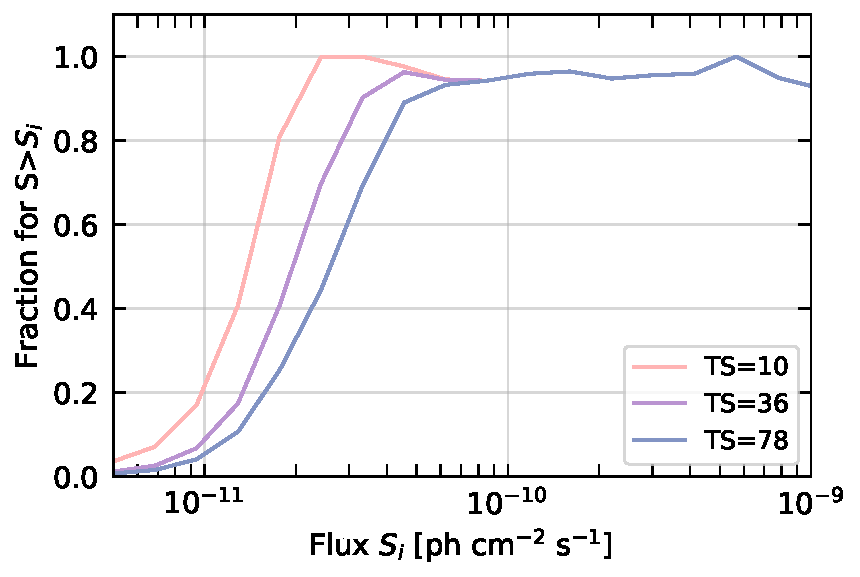
\includegraphics[width=0.6\textwidth]{chapter_07/paper_dnds_catalog/img/pixel_firing_4FGL_cumul_10_36_78.pdf}
\caption{Fraction of sources in the model $\mathcal{K}$ map, whose position corresponds to  a firing pixel for different values of $TS$. See text for details.}
\label{fig:2}
\end{figure}

In figure~\ref{fig:2} we compute, as a function of the flux, the fraction of all the pixels in the catalogue map $\mathcal{K}$, having a flux $S>S_i$, which coincide with the pixels of our  firing pixels map obeying the same flux condition, for different $TS$ cuts. The pixel coincidence is actually relaxed to a distance corresponding to the 68\% containment angle of the PSF, which naively accounts for the uncertainty of the quoted source centroids in the 4FGL catalogue.  
In figure~\ref{fig:2} we compute the fraction of all the pixels in the catalogue map $\mathcal{K}$ with flux $S>S_i$, whose positions are found in spatial coincidence with  pixels in our firing-pixels map obeying the same flux condition.\footnote{The pixel-wise spatial coincidence is actually relaxed to a distance corresponding to the 68\% containment angle of the PSF, which naively accounts for the uncertainty of the quoted source centroids in the 4FGL catalogue.} We display the fraction as a function of the flux and for different $TS$ cuts. 


\begin{figure}[t]
\centering
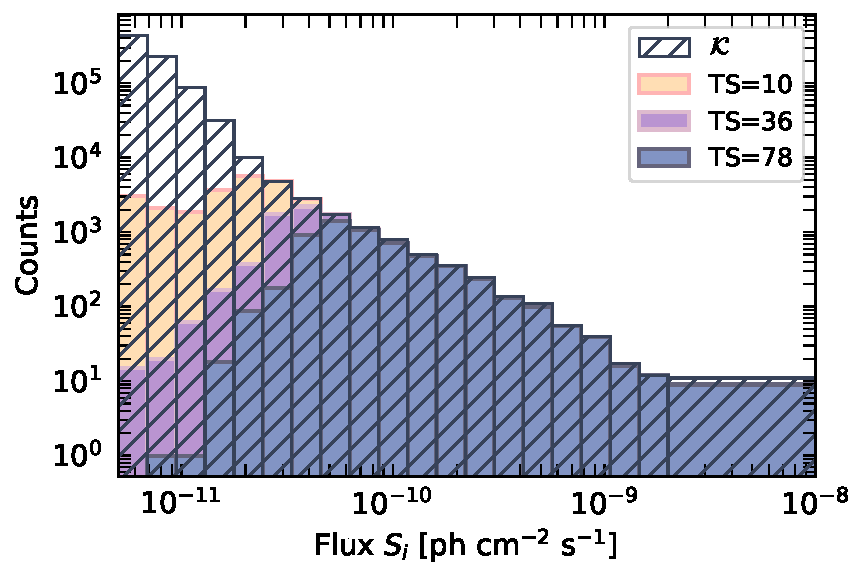
\includegraphics[width=0.6\textwidth]{chapter_07/paper_dnds_catalog/img/pixel_firing_4FGL_all_log.pdf}
\caption{Analogous to  figure~\ref{fig:2}, but for differential flux; i.e. number of pixels for a given flux bin. White histograms correspond to the whole catalogue map $\mathcal{K}$, while colored histograms are only those pixels in $\mathcal{K}$ coinciding (within the 68\% PSF containment angle) with the firing pixels of our \dNdS~model map. }
\label{fig:2b}
\end{figure}

Roughly~\footnote{More quantitative considerations require energy- and position-dependent assessments.}, \Fermi-LAT starts to loose sensitivity to sources below $2\times 10^{-10}\, \textrm{cm}^{-2}\textrm{s}^{-1}$~\cite{Zechlin:2015wdz,DiMauro:2017ing,Marcotulli:2020fpm,Amerio:2023uet}, above the rising region of the sigmoid-like curves of figure~\ref{fig:2}. As expected, modulo fluctuations, the fraction tends towards unity at high fluxes. Note that we do not expect perfect recovering of the sources in the \Fermi-LAT catalogue, anyway, either due to some simplifications (e.g.~we use energy-integrated quantities for our analysis, as opposed to the differential energy analysis by the LAT collaboration) or methodological differences, such as the pixelisation procedure or the iterative background estimate procedure in \Fermi. But it is clearly the case that we do recover the largest majority of the ``bona fide'' sources that we should. 

%
Figure~\ref{fig:2b} gives us a more detailed look at the information contained in figure~\ref{fig:2}. In this case we do not consider the ``cumulative'' number of pixels, but only those lying in a certain flux bin. The colored histograms correspond to the pixels in map $\mathcal{K}$ matching with the firing pixels of our \dNdS~model map (related to the numerator of the fraction computed in figure~\ref{fig:2}). The white histogram instead correspond to all the pixels in map $\mathcal{K}$ (related to the denominator of the aforementioned fraction). The sigmoid curve in figure~\ref{fig:2} grows close to unity at large $S$ since---barring fluctuations---the quasi-totality of sources in the catalogue are found within the adopted cuts. When lowering the cut $TS$, the peak of the colored histogram shifts to lower $S$, while still preferentially populating the high-$S$ tail (compare case $TS=36$ with case $TS=78$). If the $TS$ is lowered too much, as illustrated by the case $TS=10$, the matching starts developing a ``flat tail'' at lower $S$, hinting at a growing  random match component. Eventually, the curves in figure~\ref{fig:2} drop to zero at low $S$ not because of the scarcity of matchings (i.e., the numerator), but due to the faster growing number of pixels having flux above the indicated value (i.e. the denominator).

As a further check, we assess how  robust the selected catalogue is to variations of the background model. We compare the results obtained with the \verb|gll_iem_v07| template with the previous incarnation of the galactic foreground model developed by the Fermi collaboration: \verb|gll_iem_v05_rev1|. Since the $TS^*$ scale and related $QF$ are quantitatively different if the different backgrounds are used, we proceed by comparing the two results \textit{at equal number of selected sources}.  We select $TS^*$ cuts delivering the same number of selected sources for the two cases and evaluate the exact overlap of pixel candidates. The results are reported in Table~\ref{tab:bck_comp}. As can be seen, within a few percent, the catalogues obtained agree.


\begin{table}[t]
    \renewcommand{\arraystretch}{1.2}
    \centering
    \begin{tabular}{|c|c|}  
    \hline
        N &  coincidence  \\
        \hline 
       3000 & 98.4\% \\
        \hline 
       5000 & 97.8\% \\
        \hline 
       9000 & 97.8\% \\
       \hline
    \end{tabular}
\caption{The fraction of firing pixels in common between the selections derived for the two galactic foreground models. The comparison is performed at equal number of selected sources for the two cases.}  
\label{tab:bck_comp}
\end{table}


The main output of our work consists of sky maps of ``firing'' pixels (i.e.~source candidates). These pixels have a significant $TS$ value among all pixels for which there is a statistical compatibility between simulations and real data, according to KS tests. The firing pixels depend on the significance $\alpha$ of the KS test, as well as on a ``quality factor'' $QF$, accounting for the fraction of simulated maps passing the KS test.
We provide our results electronically in the form of a Python package called \verb|gPCS|  (for gamma-ray Photon Count Statistics), as well as a summary \verb|FITS|, both available on Zenodo: \href{https://doi.org/10.5281/zenodo.8070852}{https://doi.org/10.5281/zenodo.8070852}. The Python package can be used to determine the firing pixels given either a $TS_*$ or a quality factor and $\alpha$ parameter. The Python package also includes a convenience function to export the firing pixels in the form of a \verb|FITS| file, and we provide an example on how to compute the summary table provided with the package.
\\
The \verb|gPCS| Python package can be easily installed using \verb|pip|, with the command:
\begin{lstlisting}[language=Python]
pip install gPCS
\end{lstlisting}
In order to get the firing pixels, given either $TS_*$ or a quality factor and $\alpha$, we can use the following snippet of code:

\begin{lstlisting}[language=Python]
import numpy as np
from gPCS import gPCS

# specify manually a TS_star
TS_star = 36
pixel_firing = gPCS.get_firing_pixels(TS_star, filter=False)
print(len(pixel_firing))

# Compute the TS_star from a chosen QF and alpha
# [alpha must be 0.01, 0.05 or 0.1]
QF = 0.5
alpha = 0.05
TS_star = gPCS.get_TS_from_QF(QF, alpha=alpha)
pixel_firing = gPCS.get_firing_pixels(TS_star, filter=False)
print(len(pixel_firing))
\end{lstlisting}
It is possible to export a \verb|FITS| table using the \verb|export_fits_table| function. For example to reproduce the table provided with the library we can use:

\begin{lstlisting}[language=Python]
gPCS.export_fits_table(filename="firing_pixels.fits", QF=0.50, alpha=[0.01, 0.05, 0.1])
\end{lstlisting}
The \verb|FITS| table has the following fields:
\begin{lstlisting}[basicstyle=\ttfamily]
    pixel   : pixel index
    TS      : TS value for each pixel
    QF_best : QF value obtained by considering all the simulations
    QF_min  : lower bound of the QF range
    QF_max  : upper bound of the QF range
\end{lstlisting}
For further details on the package usage, please refer to the documentation and examples: \\
\href{https://github.com/aurelio-amerio/gPCS}{https://github.com/aurelio-amerio/gPCS}.






%%%%

